\section{Presheaves and the Yoneda lemma}

For references for this section see \cite[Section 4.2 \& 4.3]{LeinBasi2014}.

Throughout we will fix a small category $\mathcal{A}$.

\begin{defi}
    Let $\widehat{\mathcal{A}}\coloneqq \Fun(\mathcal{A}^{\op},\Set)$ be the category of contravariant functors from $\mathcal{A}$ to the category of sets.
    This category will be called the category of \underline{presheaves} on $\mathcal{A}$.
    By definition $X \in \widehat{A}$ consists of the following data:
    \begin{itemize}
        \item 
        $\forall a \in \mathcal{A} \text{ a set } X_a \coloneqq X(a) \in \Set$
        This set will be called the \underline{fibre} of $X$ at $a$.
        \item 
        $\forall u\colon b \to a\in \widehat{\mathcal{A}}(b,a)$ a map of sets $u^*=X(u)\colon X_a \to X_b$ such that functoriality constraints are satisfied:
        \item 
        (Unitality) For all objects $a \in \mathcal{A}$ a morphism $(\id_a)^*=X(\id_a)\colon X_a \to X_a$ such that $(\id_a)^*=\id_{X_a}$.
        \\
        (Composition) For all composition of morphisms in $\mathcal{A}$ a composition of the induced morphisms on the fibres:
        \[
            \begin{tikzcd}
                a
                \arrow{r}[above]{u}
                \arrow[rr, bend right, "v \circ u"']
                &
                b
                \arrow{r}[above]{v}
                &
                c
            \end{tikzcd} 
            \qquad
            \begin{tikzcd}
                &
                X_b
                \arrow[dl, "u^*"']
                &
                \\
                X_a 
                &
                &
                X_c
                \arrow[ul,"v^*"']    
                \arrow[ll,"(v \circ u)^*"]
            \end{tikzcd}
        \]
        which is equivalent to $u^* \circ v^* = (v \circ u)^*$.
    \end{itemize}
\end{defi}

\begin{rmk}
    Throughout we are going to talk alot alot about presheaves, especially representable ones, what happens when we introduce sheaves and maybe use sheaves in the later theory.
\end{rmk}

\begin{exmp}
    Let $M$ be a monoid, then $BM$ is the category with a single object $\Ob(BM) \coloneqq \{*\}$ and morphisms $BM(*,*) \times BM(*,*) \to BM(*,*)=M$.
    A presheaf $X \in \widehat{BM}$ consists of a set $X=X_* \in \Set$ and for each $m \in M$ a morphism $m^*: X \to X$ that we denote on elements by left multiplication $m^*(x)=x \cdot m$.
    Moreover a morphism $e_m^*\colon X \to X$ such that $e_m^*=\id_{X^*}$, that is $x \cdot e_M=x$ for all $x \in X$.
    At last for any diagram of morphisms in $BM$, a diagram in $\Set$
    \[
    \begin{tikzcd}
        &
        *
        \arrow[rd,"u"]
        &
        \\
        *
        \arrow[ru,"m"]
        \arrow[rr,"um"']
        &
        &
        *
    \end{tikzcd}
    \qquad
    \begin{tikzcd}
        &
        X
        \arrow[ld,"\cdot m"']
        &
        \\
        X
        &
        &
        X
        \arrow[lu,"\cdot u"']
        \arrow[ll,"\cdot (um)"]
    \end{tikzcd}
    \]
    which means that $x\cdot (nm)=(xn)\cdot m$.
\end{exmp}

\begin{defi}
    For every $a\in \mathcal{A}$, let $\mathcal{A}$ be the functor,
    \[
    \begin{tikzcd}
        \mathcal{A}(-,a)\colon \mathcal{A}^{\op}
        \arrow[r]
        &
        \Set
        \\
        b
        \arrow[r, mapsto]
        &
        \mathcal{A}(b,a)
        \arrow[d,"u^*"]
        &
        b \xrightarrow{v} a
        \\
        c
        \arrow[u,"u"]
        \arrow[r, mapsto]
        &
        \mathcal{A}(c,a)
        &
        c \xrightarrow{u} b \xrightarrow{v}a
    \end{tikzcd}
    \]
    is the presheaf represented by a $\in \mathcal{A}$.
\end{defi}

Let $X,Y \in \widehat{\mathcal{A}}$ be presheaves. 
By definition a morphism $f\colon X \to Y$ is a natural transformation of functors $\eta \colon \mathcal{A}^{\op} \to \Set$, that is for every $a \in \mathcal{A}$ a morphism of sets $\eta_a:X_a \to Y_a$ such that the usual naturality constraint holds, that is 
    \[
    \begin{tikzcd}
        a
        \arrow[d, "u"]
        & 
        X_a
        \arrow[r, "\eta_a"]
        & 
        Y_a
        \\
        b
        &
        X_b
        \arrow[u,"u^*"]
        \arrow[r, "\eta_b"]
        &
        Y_b
        \arrow[u,"u^*"']
    \end{tikzcd}
    \]
commutes for every morphism $u$ in $\mathcal{A}$, so we have $u^* \circ \eta_b = \eta_a \circ u^*$.

\begin{exmp}
    Let $M$ be a monoid and $X,Y \in \widehat{BM}$.
    A morphism $f\colon X \to Y $ consists of a function $f=f^*\colon X =X_* \to Y_*=Y$ such that, the following diagram commutes
    \[
    \begin{tikzcd}
        *
        \arrow[d,"m"]
        &
        X
        \arrow[r,"f"]
        &
        Y
        \\
        *
        &
        X
        \arrow[u,"m"]
        \arrow[r,"f"]
        &
        Y
        \arrow[u,"m"']
    \end{tikzcd}
    \]
    for $m\in BM(*,*)$.
\end{exmp}

\begin{thm}{Yoneda lemma version 1}
\label{yoneda_lemma}
    Let $a$ be an object in $\mathcal{A}$ and $X \in \widehat{\mathcal{A}}$ a presheaf.
    Then 
    \[
    \begin{tikzcd}
       \phi = \phi_{a,x}\colon\Hom_{\widehat{\mathcal{A}}}(\mathcal{A}(-,a),X) 
       \arrow[r]
       &
       X_a 
       \\
       f 
       \arrow[r,mapsto]
       &
       f_a(\id_a)
    \end{tikzcd}
    \]
    is bijective.
\end{thm}

\begin{proof}
    We first observe that the following square commutes
    \[
    \begin{tikzcd}
        b
        \arrow[d,"u"]
        &
        \mathcal{A}(b,a)
        \arrow[r,"f_b"]
        &
        X_b
        \\
        a
        &
        \mathcal{A}(a,a)
        \arrow[u,"u^*"]
        \arrow[r,"f_a"]
        &
        X_a
        \arrow[u,"u^*"']
    \end{tikzcd}
    \]
    which means $f_b(u^*(\id_a))=f_b(u)=u^*(f_a(\id_a))=u^*(\phi(f))$.
    So without evaluating at an object we get $f_b(-) = (-)^*(\phi(f))=X(-)(\phi(f))$.
    Let us first show that $\phi$ is injective, suppose $f,g\colon\mathcal{A}(-,a) \to X$ such that $\phi(f)=\phi(g)$.
    For $b \in \mathcal{A}$ we get morphisms $f_b,g_b\colon\mathcal{A}(b,a) \to X_b$ and for any morphism $u:b\to a$ in $\mathcal{A}$ we get that $f_b(u)=u^*(\phi(f))=u^*(\phi(g))=g_b(u)$ and thus $f=g$.
    Let us now show that $\phi$ is surjective.
    Let $x \in X_a$ and $f^\times\coloneqq ( f_b^\times\colon \mathcal{A}(b,a) \to X_b \mid b \in \mathcal{A})$ given on any morphism $u\colon b \to a$ by $u^*(x)$.
    We need to prove that these are indeed the components of a natural transformation $f\colon \mathcal{A}(-,a) \to X$.
    \[
    \begin{tikzcd}
        b
        \arrow[d,"u"]
        &
        \mathcal{A}(b,a)
        \arrow[r,"f_b^\times"]
        &
        X_b
        \\
        a
        &
        \mathcal{A}(c,a)
        \arrow[u,"u^*"]
        \arrow[r,"f_a^\times"]
        &
        X_c
        \arrow[u,"u^*"']
    \end{tikzcd}
    \]
    The square commutes, which gives for any $c \xrightarrow{\nu} a$ in $\mathcal{A}$, that 
    \begin{center}
        $f_b^\times(u^*(\nu)) = f_b^\times(\nu \circ u) = ( \nu \circ u)^*(x) =u^*(f^\times_c(\nu)) = $
        \\
        $u^*(\nu^*(x))=(u^* \circ \nu^*)(x)= (\nu \circ u)^*(x)$.
    \end{center}
\end{proof}

Lecture 3 15.10

\begin{thm}
\label{yoneda_embedding}
    The functor $\mu: \mathcal{A} \to \widehat{\mathcal{A}}$
    \[
    \begin{tikzcd}
        a
        \arrow[r,mapsto]
        \arrow[d]
        &
        \widehat{a}=\mathcal{A}(-,a)
        \arrow[d,"\widehat{u}"]
        &
        \mathcal{A}(c,a)
        \arrow[d,"\widehat{u}_c"]
        \\
        b
        \arrow[r,mapsto]
        &
        \widehat{b}=\mathcal{A}(-,b)
        &
        \mathcal{A}(c,b)
    \end{tikzcd}
    \]
    that sends an object of $a$ to the the presheaf of morphisms into $a$ is fully faithfull called the \underline{Yoneda embedding}.
\end{thm}

\begin{proof}
    We first have to show that $\mu$ is a functor. 
    So let $u\colon a \to  b$ be a morphism.
    The claim is that $\widehat{u}\colon \widehat{a} \to \widehat{b}$ is a natural transformation.
    \[
    \begin{tikzcd}
        c
        \arrow[d,"v"]
        &
        \mathcal{A}(c,a)
        \arrow[r,"u_*"]
        &
        \mathcal{A}(c,b)
        \\
        d
        &
        \mathcal{A}(d,a)
        \arrow[u,"\nu^*"]
        \arrow[r,"u_*"]
        &
        \mathcal{A}(d,b)
        \arrow[u,"\nu^*"']
    \end{tikzcd}
    \]
    The square commutes, which means that morphisms are mapped to natural transformations under $\mu$, thus $\mu$ is actually a functor.
    Next let us show that $\mu$ is fully faithfull, which means that the $\mu$ is a bijection on hom-sets
    \[
    \begin{tikzcd}
        \mu \colon \mathcal{A}(a,b) 
        \arrow[r]
        &
        \Hom_\mathcal{\widehat{A}}(\widehat{a}, \widehat{b}).
        \arrow[l, bend right, dashed, "\phi"']
    \end{tikzcd}
    \]
    We claim that
    \[
    \phi \circ \mu = \id.
    \]
    Let $u\colon a \to b$, then
    \[
    \phi(\widehat{u}) = \widehat{u}_a(\id_a) = u \circ \id_a = u
    \]
    which proves the above claim.
\end{proof}

\begin{rmk}
    There is the contravariant Yoneda embedding as well, given by
    \[
    \begin{tikzcd}
        \mu_{\mathcal{A}^{\op}} \colon \mathcal{A}^{\op}
        \arrow[r]
        &
        \widehat{\mathcal{A}}^{\op} = \Fun(\mathcal{A}, \Set)
        \\
        a 
        \arrow[r, mapsto]
        &
        \mathcal{A}^{\op}(-,a)= \mathcal{A}(a,-).
    \end{tikzcd}
    \]
\end{rmk}

\begin{prop}
    Let $X \in \widehat{\mathcal{A}} $ consider the presheaf
    \[
    \begin{tikzcd}
        \Hom_{\widehat{\mathcal{A}}}(\mathcal{A}(-,?) , X ) \colon \mathcal{A}^{\op} 
        \arrow[r]
        &
        \Set
        \\
        \mathcal{A}
        \xhookrightarrow{\mu}
        \widehat{A}
        \arrow[r, "\Hom_{\widehat{\mathcal{A}}}{( -, X )}"]
        &
        \Set
        \\
        a \mapsto \mathcal{A}(-,a)
        \arrow[r, mapsto]
        &
        \Hom_{\widehat{\mathcal{A}}}(\mathcal{A}(-,a),X)
    \end{tikzcd}
    \]
    Then 
    \begin{align*}
    	\phi_{?,X}: \Hom_{\widehat{\mathcal{A}}}(\mathcal{A}(-,?),X) 
    	&\to 
    	X
    	\\
	    \phi_{?,X}=(\phi_{a,X}\colon\Hom_{\widehat{\mathcal{A}}}(\mathcal{A}(-,a),X) 
	    &\isomorphism 
	    X_a \mid a \in \mathcal{A})
    \end{align*}
    is a natural isomorphism of presheaves.
\end{prop}

\begin{proof}
    We only need to prove naturality since $\phi_{a,X}$ is an isomorphism for every $a$ by \cref{yoneda_lemma}.
    So let us look at the following square
    \[
    \begin{tikzcd}
        a 
        \arrow[d, "u"]       
        &
        \Hom_{\widehat{\mathcal{A}}}(\mathcal{A}(-,a),X) 
        \arrow[r , "\phi"]
        &
        X_a
        \\
        b 
        &
        \Hom_{\widehat{\mathcal{A}}}(\mathcal{A}(-,b),X) 
        \arrow[r, "\phi"]
        \arrow[u,"? \circ \widehat{u}"]
        &
        X_b
        \arrow[u, "u^*"']
    \end{tikzcd}
    \]
    For $f\colon \widehat{b} \to X$ the commutative square yields
    \[
    \begin{tikzcd}
        &
        u^*(f_b(\id_b))=f_a(u)
        \\
        f
        \arrow[r]
        &
        f_b(\id_b)
        \arrow[u, mapsto]
    \end{tikzcd}
    \qquad
    \begin{tikzcd}
        (f \circ \widehat{u})
        \arrow[r]
        &
        (f \circ \widehat{u})_a(\id_a)
        \\
        f
        \arrow[u, mapsto]
    \end{tikzcd}
    \]
    where $f_a \colon \mathcal{A}(a,b) \xrightarrow{f_a}X_a$.
    Notice that $ (f\circ\widehat{u})_a(\id_a) = f_a \circ \widehat{u}_a ( \id_a) = f_a ( u \circ \id_a) = f_a(u)$ which means both compositions 
    are the same, so the square commutes. 

\end{proof}

\begin{defi/prop}
    Let $X\in \widehat{\mathcal{A}}$ then the following are equivalent:
    \begin{enumerate}
        \item 
        There $\exists a \in \mathcal{A}$ such that $\exists f \colon \widehat{a} \to X $ that is an isomorphism in $\widehat{\mathcal{A}}$.
        \item 
        $\exists a \in \mathcal{A}$ and $\exists x \in X_a$ such that $\forall b \in \mathcal{A}$, we have that
        \[
        \begin{tikzcd}
            \mathcal{A}(b,a) \to X_b 
             &
             u \mapsto u^*(x)
        \end{tikzcd}
        \]
        is an isomorphism.
        \item 
        There $\exists a \in \mathcal{A}$ and $\exists x \in X_a$ such that $\forall b \in \mathcal{A}$ and $\forall u \in \mathcal{A}(b,c)$ we have that $\exists! y\in X_b$ such that $u^*(x)=y$.
    \end{enumerate}
    We call the pair $(a \in \mathcal{A}, x \in X_a)$ a \underline{representation} of $X$ and $a\in \mathcal{A}$ a \underline{representing object} and $x \in X_a$ a \underline{universal element}.
\end{defi/prop}

\begin{proof}
    This can be deduced from the previous proposition.
\end{proof}

\begin{prop}
    For an element $a \in \mathcal{A}$ the isomorphism $\phi_{a,X} \colon \Hom_{\mathcal{\widehat{A}}}(\widehat{a},X) \isomorphism X$ is natural in $X$.
\end{prop}

\begin{proof}
    Consider the following commutative diagram 
    \[
    \begin{tikzcd}
        X
        \arrow[d,"f"]
        & 
        \Hom_{\widehat{\mathcal{A}}}(\widehat{a},X) 
        \arrow[r, "\phi"]
        \arrow[d, "f \circ ?"]
        &
        X_a
        \arrow[d,"f_a"]
        \\
        Y
        &
        \Hom_{\widehat{\mathcal{A}}}(\widehat{a}, Y) 
        \arrow[r, "\phi"]
        &
        Y_b
    \end{tikzcd}
    \]
    which evaluates on an element $g \colon \widehat{a} \to X$ to
    \[
    \begin{tikzcd}
        g
        \arrow[r,mapsto]
        &
        \phi(g) = g_a (\id_a)
        \arrow[d,mapsto]
        \\
        &
        f_a(g_a(\id_a))          
    \end{tikzcd}
    \qquad
    \begin{tikzcd}
        g
        \arrow[d,mapsto]
        &
        \\
        (f \circ g)
        \arrow[r, mapsto]
        & 
        \phi(f \circ g)=(f \circ g)_a(\id_a)
    \end{tikzcd}
    \]
    comparing the two outcomes, we get the following equalities
    \[
    f_a(g_a(\id_a))= (f_a \circ g_a)(\id_a) =(f \circ g)_a (\id_a)
    \]
    which yields the result.
\end{proof}

\begin{thm}{The Yoneda lemma}
    Let $\mathcal{A}$ be a small category. The functions 
    \[
    \begin{tikzcd}
        \phi_{a,X}\colon \Hom_{\widehat{\mathcal{A}}}(\widehat{a},X) 
        \arrow[r,"\phi"]
        &
        X_a
        \\
        f
        \arrow[r,mapsto]
        &
        f_a(\id_a)
    \end{tikzcd}
    \] 
    are natural in $a \in \mathcal{A}^{\op}$ and $X \in  \widehat{\mathcal{A}}$ seperately.
    Hence they yield an isomorphism of functors.
    \[
    \begin{tikzcd}
        \mathcal{A}^{\op} \times \widehat{\mathcal{A}}
        \arrow[rr, bend left , "\Hom_{\presh{A}}{(\mu(?),-)}" pos=0.45]
        \arrow[rr , bend right , "\ev"' pos=0.5325]
        &
        \Downarrow
        &
        \Set
    \end{tikzcd}
    \]
    Given on and object $(a,X)$ as follows.
    \[
    \begin{tikzcd}
        & 
        \Hom_{\presh{A}}(\widehat{a},X)
        \arrow[dd,"\phi_{(a,X)}"]
        \\
        (a,X)
        \arrow[rd, mapsto]
        \arrow[ru, mapsto]
        &
        \\
        &
        X_a
    \end{tikzcd}
    \]
\end{thm}

\subsection{ Exercises }

\begin{Exercise}
    Alice and Bob are randomly placed in a $ 3 \times 2 $-grid on two different squares.
    \begin{center}
        \begin{tikzpicture}
            \draw (-3,2) -- (3,2);
            \draw (-3,-2) -- (3,-2);
            \draw (-3,0) -- (3,0);
            \draw (-3,-2) -- (-3,2);
            \draw (-1,-2) -- (-1,2);
            \draw (1,-2) -- (1,2);
            \draw (3,-2) -- (3,2);
            \node[red, scale = 2] (B) at (2,1) {B};
            \node[blue, scale = 2] (A) at (-2,-1) {A};
        \end{tikzpicture}
    \end{center}
    
    Every turn they are moving to an orthogonally adjacent square which is not currently occupied and they never move to the same square.
    
    \begin{enumerate}[label=(\alph*)]
    
        \item 
        Describe the groupoid of configurations by connecting two configurations if they are connected by a single turn.  
        
        \item 
        Which of the following configurations can be reached from the above? 
        How many connected components does the groupoid have?
        \begin{center}
            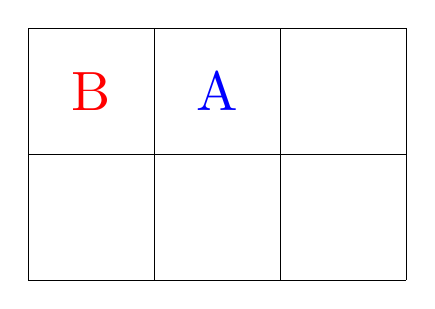
\begin{tikzpicture}[scale = 0.8]
                \draw (-3,2) -- (3,2);
                \draw (-3,-2) -- (3,-2);
                \draw (-3,0) -- (3,0);
                \draw (-3,-2) -- (-3,2);
                \draw (-1,-2) -- (-1,2);
                \draw (1,-2) -- (1,2);
                \draw (3,-2) -- (3,2);
                \node[red, scale = 2] (B) at (-2,1) {B};
                \node[blue, scale = 2] (A) at (0,1) {A};
            \end{tikzpicture}
            \qquad
            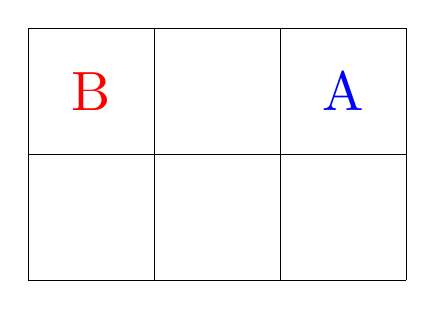
\begin{tikzpicture}[scale = 0.8]
                \draw (-3,2) -- (3,2);
                \draw (-3,-2) -- (3,-2);
                \draw (-3,0) -- (3,0);
                \draw (-3,-2) -- (-3,2);
                \draw (-1,-2) -- (-1,2);
                \draw (1,-2) -- (1,2);
                \draw (3,-2) -- (3,2);
                \node[red, scale = 2] (B) at (-2,1) {B};
                \node[blue, scale = 2] (A) at (2,1) {A};
            \end{tikzpicture}
        \end{center}
    
        \item 
    
        Describe what additional information the groupoid holds over the equivalence classes of configurations up to moves.
        
    \end{enumerate}
\end{Exercise}

\begin{Exercise}
    For an (associative and unital) ring $ R $ let $ B R $ be the category associated to the multiplicative monoid of $ R $.
    Show that there is an isomorphism of categories $ \psi \colon \Mod_R \to \Fun_{ \mathbb{ Z } } ( ( B R )^{ \op } , \Ab ) $ relating the category of right $ R $-modules into the category of '$ \mathbb{ Z } $-linear presheaves over $ B M $', i.e. contravariant $ \mathbb{ Z } $-linear functors from $ B R $ to the category of abelian groups $ \Ab $.
\end{Exercise}


\begin{Exercise}
    Let $ R $ be a ring and let $ \prescript{  }{ R }{ R }_R$ be $ R $ viewed as an $ R $-$ R $-bimodule.
    
    \begin{enumerate}[label=(\alph*)]
    
        \item 
        Show that for any $ R $-$ R $-bimodule $ N $ and any $ M \in \mod_R $ that $ \Hom_{ \mod R } ( N , M ) $ carries the structure of a right $ R $-module via $ ( f r ) ( x ) \coloneqq f ( r x ) $. 
        Deduce that $ N $ induces a functor
        \[
            \Hom_{\mod R } ( N , - ) \colon \mod R \to \mod R.
        \]
        
        \item 
        
        Show that there is an isomorphism of functors $ \Hom_{ \mod R } ( \prescript{}{ R }{ R }_R , - ) \cong \id_{ \mod R } $ given by evaluation at $ 1 \in R $.
    \end{enumerate}
\end{Exercise}

\begin{Exercise}
    Consider four sets $ A , B , C $ and $ E $ and assume that $ A , B \subseteq C $ with the inclusions $ \iota_A $ and $ \iota_B $.
    
    \begin{enumerate}[label=(\alph*)]
        \item 
        Show that for any two maps $ \phi_A \colon E \to A $ and $ \phi_B \colon E  \to B $ such that $ \iota_A \circ \phi_A = \iota_B \circ \phi_B $ there is a unique map $ \phi \colon E \to A \cap B $ such that $ \phi_A = i_A \circ \phi $ and $ \phi_B = i_B \circ \phi $ for $ i_A $ and $ i_B $ the respective inclusions of $ A \cap B $. 
        \[
        \begin{tikzcd}
            E 
            \ar[rd, dashed, " \exists ! \phi" ]
            \ar[rrd, bend left, " \phi_A" ]
            \ar[rdd, bend right, " \phi_B" ']
            \\
            &
            A \cap B
            \ar[r , " i_A " ]
            \ar[d , " i_B " ]
            &
            A
            \ar[ d , " \iota_A" ]
            \\
            &
            B
            \ar[r, " \iota_B " ]
            &
            C
        \end{tikzcd}
        \]
    
        \item 
        Give an example of two maps $ f_A \colon A \to D $ and $ f_B \colon B \to D $ such that $ A \cap B $ does not have the above property for $ f_A $ and $ f_B $ instead of $ \iota_A $ and $ \iota_B $.
    
        \item 
        Show that in this more genral setting that
        \[
            A \times_D B \coloneqq \{ ( a, b ) \in A \times B \mid f_A ( a ) = f_B ( b ) \}
        \]
        with the canonical projections $ p_A, p_B$ satisfying the universal property from before.
        \[
        \begin{tikzcd}
            E 
            \ar[rd, dashed, " \exists ! \phi" ]
            \ar[rrd, bend left, " \phi_A" ]
            \ar[rdd, bend right, " \phi_B" ']
            \\
            &
            A \times_D B
            \ar[r , " p_A " ]
            \ar[d , " p_B " ]
            &
            A
            \ar[ d , " f_A" ]
            \\
            &
            B
            \ar[r, " f_B " ]
            &
            D
        \end{tikzcd}
        \]
    
        \item 
        What is the relation between $ A \cap B $ and $ A \times_C B$ for part (a)?
    \end{enumerate}
\end{Exercise}
    


